The dynamics of the electrons
discussed in \cref{sec:the model}
can be investigated by
directly simulating the system.

\subsection{Eigenvalue Decomposition}
To simulate the system we must solve
the Schrödinger equation. This
can be done through direct
integration, however
if we first decompose
the initial state
into eigenstates
of the complete hamiltonian\cite{conduit}
\begin{align}
    \ket{\Psi(t)} = \exp{(-i\frac{Ht}{\hbar})} \sum_n C_n \ket{n} \\
    = \sum_n C_n \exp{(-i\frac{E_n t}{\hbar})} \ket{n}
\end{align}
we can propagate
by multiplying each eigenstate
by a phase-factor.

Since we are dealing with a
large number of eigenstates
it is important to think
about both the storage
and computational complexity
of the two methods (\cref{tab:algorithm complexity}).
\begin{table}[htbp]
    \begin{center}
        \begin{tabular}{ *{3}{c} }
            \toprule
            Cost    & Integration            & Decomposition              \\
            \midrule
            Time    & \(\mathcal{O}(n^2 t)\) & \(\mathcal{O}(n^3 + n d)\) \\
            Storage & \(\mathcal{O}(n d)\)   & \(\mathcal{O}(n^2 + n d)\) \\
            \bottomrule
        \end{tabular}
    \end{center}
    \caption{Complexity associated with the
        two methods of solving Schrödinger equation,
        where \(n\) is the number of eigenstates, t
        is the number of timesteps and d is the
        number of datapoints. The method
        of eigenvalue decomposition
        prevents the \(\mathcal{O}(t)\)
        dependence seen
        in direct integration
        by first decomposing the
        eigenstate (\(\mathcal{O}(n^3)\))
        before multiplying
        by the relevant phase
        (\(\mathcal{O}(nd)\)).
    }\label{tab:algorithm complexity}
\end{table}

As we
are only interested in the
evolution of the eigenstates
at times much greater than
the frequency of the sates
\(\omega = \frac{E}{\hbar}\)
the method of integration
was found to be much
slower than that of eigenvalue
decomposition. One
issue with this method
is the increased storage
cost associated with
storing the complete
hamiltonian. This could
be prevented by
working with a sparse
matrix, however in
practise this
was not required.

Although the decomposition is
expensive it was only repeated once,
which allowed us to gather a large
number of times at very little additional
cost. It was also possible to use the
fact that the matrix was hermitian to
provide and additional increase in speed.

\subsection{Matrix Representation}\label{sec:state representation}
Working in the unperturbed electron basis
(\cref{sec:electron states})
we label each eigenstate
according to the index of the
hydrogen site and
the configuration of the
electron system.
In general for \(n\)
electron states
and \(m\) hydrogen states
there would
be \(m 2^n\)
possible configurations,
however since the hamiltonian
conserves particle number
we limit ourselves
to a fixed
number of electrons (\(N\)).
In this case the number
of states scales as \(m \times{} \binom{n}{N}\).
In practise we are able to
simulate a system with
around \(3500\) eigenstates,
or \(14\) half filled electron states
(\cref{tab:number of eigenstates}).
This was limited more by
storage than CPU time, and as such it may
be necessary to investigate
the use of sparse matrices if a
larger system is required.
\begin{table}[htbp]
    \begin{center}
        \begin{tabular}{ *{4}{c} }
            \toprule
            Number of States & All Configurations & Half Filled & 2 electrons \\
            \midrule
            \(10\)           & \(1024\)           & \(252\)     & \(45\)      \\
            \(12\)           & \(4096\)           & \(924\)     & \(66\)      \\
            \(14\)           & \(16384\)          & \(3432\)    & \(91\)      \\
            \(16\)           & \(65536\)          & \(12870\)   & \(120\)     \\
            \bottomrule
        \end{tabular}
    \end{center}
    \caption{
        Number of eigenstates required
        to store an electron system.
        Limiting ourselves to
        configurations with a fixed
        number of electrons we are
        able to simulate a larger
        number of states.
        This method scales particularly
        well for a system with a
        low number of electrons
        or a low number of holes.
    }\label{tab:number of eigenstates}
\end{table}

The process of converting
between these labels and
the states used in the hamiltonian
was handled by
an ElectronSystem object (TODO reference)


When working with
fermions we need to take
care over the exchange
statistics of the hamiltonian.
For self consistency we work in
a basis such that electrons
with lower energy are always
added first. Terms in the interaction
hamiltonian therefore pick
up a minus sign when there is
an odd number of electrons
between the exchanged energy levels.
\begin{align}
    a^\dagger_1a_2 \ket{2,3} & = \ket{1,3}  \\
    a^\dagger_1a_3 \ket{2,3} & = -\ket{1,2}
\end{align}
To find the probability
of finding the hydrogen in site \ldots

\subsection{Choosing the Initial States}

\subsubsection{Distribution Of Energies}
The distribution of electron energies was
initially chosen using an even spacing,
however this lead noise caused
by rabi oscillations
at a frequency
fixed through several runs
of the simulation.
To remove these oscillations
random offsets were introduced
into the energy distribution
which changed the rabi frequency
between runs,
allowing for cancellation
of the noise.

The spacing of electron energies is also
important for the simulation, as it
sets the effective volume of the Nickel
lattice. The density of states of a free electron
gas \(g(E)\) is given by~\cite{KittelCharles1953Itss}
\begin{equation}
    g(E) = \frac{V}{2\pi^2}
    {(\frac{2m}{\hbar^2})}^{\frac{3}{2}}
    E^{\frac{1}{2}}
\end{equation}
We therefore invert this expression
to find the implied volume of the
simulation
\begin{equation}
    V = 2\pi^2
    \frac{g(E)}{E^{\frac{1}{2}}}
    {(\frac{\hbar^2}{2m})}^{\frac{3}{2}}
\end{equation}
Since at large \(k\)
(for \(k\sim k_f\))
the density of states is roughly
constant we make the approximation
\begin{equation}
    g(E) = \frac{dN}{dE} \sim \frac{1}{E_{space}}
\end{equation}
where \(E_{space}\) is the energy spacing
of the simulation. From \cref{eqn:simplified interacton potential} we find
\begin{equation}
    \hat{H}_{int} \propto \frac{1}{V} \propto E_{space}
    \label{eqn:energy spacing dependance of interaction hamiltonian}
\end{equation}
for smaller
energy spacing we have
a larger volume, and a smaller
perturbation.

\subsubsection{Distribution Of Electrons}
To be able to average over successive
simulations we also need to setup the
simulation with a somewhat random
choice of initial states.
We can start the hydrogen
in the FCC site by setting the
amplitudes of the HCP sites to zero
before choosing the FCC aptitudes according to
a normal distribution.

In simulations for which we choose states
with a large range of energies however
the electron distribution should not be
random and should follow the fermi dirac distribution.
To match this distribution we
need to alter the averages used
to produce the initial state vector.
Since the amplitude corresponds to
the square-root of the probability we
take the average magnitude as the
square-root of the boltzmann probability
associated with each state.
\begin{align}
    P_k & = \exp(-\beta{}E_k)     \\
    C_k & = \exp(-\beta{}E_k / 2)
\end{align}
where \(C_k\) is the wavefunction amplitude.
If we plot the resulting
electron distribution produced
by this method for fixed N
we see the expected electron
distribution for a standard electron
gas (\cref{fig:correct fermi dirac}).
\begin{figure}[htbp]
    \centering
    \begin{subfigure}{0.45\linewidth}
        \centering
        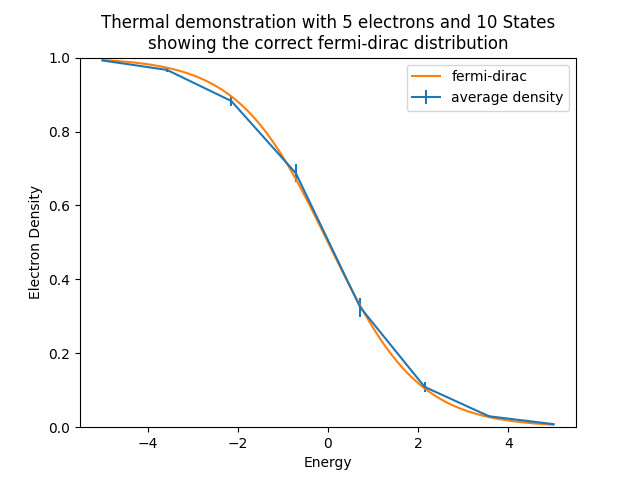
\includegraphics[width =0.9 \linewidth]{Figures/Simulation/Plot of correct fermi dirac distribution on center.png}
        \caption{5 Electrons 10 States}
    \end{subfigure}
    \hfill
    \begin{subfigure}{0.45\linewidth}
        \centering
        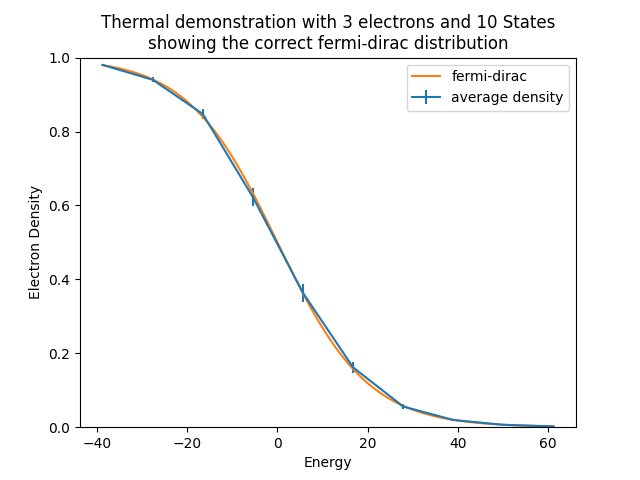
\includegraphics[width = 0.9\linewidth]{Figures/Simulation/Plot of correct fermi dirac distribution off centre.png}
        \caption{3 Electrons 10 States}
    \end{subfigure}
    \caption{Plot of the electron distribution seen
        when setting up the system randomly. The
        correct fermi-dirac distribution is seen in both the on and
        off center systems. Errors are given by the standard
        deviation of the electron densities, and are therefore
        larger around the fermi surface where fluctuations are
        large.}\label{fig:correct fermi dirac}
\end{figure}
However if we were to include
a large interaction term, such
as those required for the
real Nickel system the
electron distribution is
seen to diverge, as the approach
does not account for the
shift in the perturbed
energies (\cref{fig:incorrect fermi dirac}).
\begin{figure}[htbp]
    \centering
    \begin{subfigure}{0.45\linewidth}
        \centering
        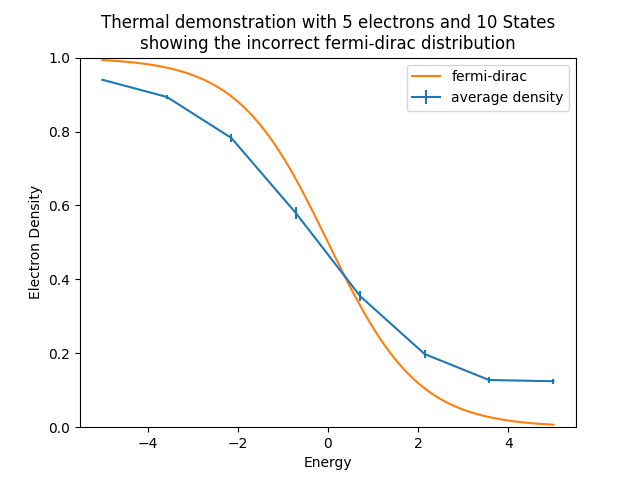
\includegraphics[width =0.9 \linewidth]{Figures/Simulation/Plot of incorrect fermi dirac distribution on center.png}
        \caption{Large interaction}
    \end{subfigure}
    \hfill
    \begin{subfigure}{0.45\linewidth}
        \centering
        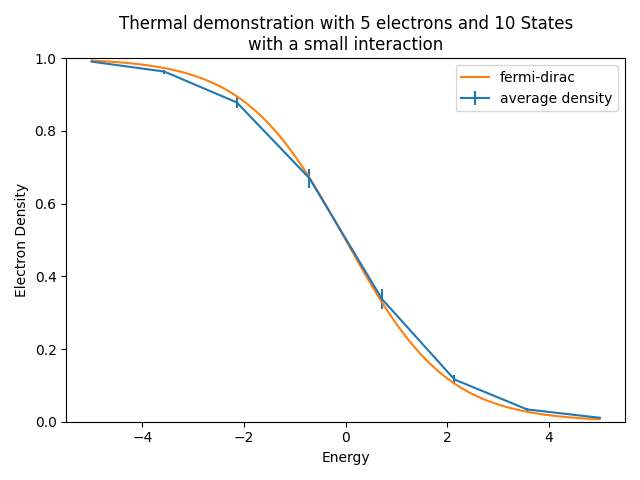
\includegraphics[width = 0.9\linewidth]{Figures/Simulation/Plot of incorrect fermi dirac distribution on center small interaction.png}
        \caption{Reduced Interaction}\label{sub@fig:reduced interaction fermi-dirac}
    \end{subfigure}
    \caption{Plot of the fermi-dirac distribution
        with the inclusion of interaction. The
        correct distribution is no longer seen when
        the full interaction is included, however
        if this is reduced by a factor of \(10\)
        (\cref{sub@fig:reduced interaction fermi-dirac})
        the correct distribution is recovered.}\label{fig:incorrect fermi dirac}
\end{figure}
To overcome this limitation
the simulation was repeated
for small energy bands (\cref{sec:small band approach})
for which the electron distribution
was uniform.

Full code is available in the appendix TODO-

\subsection{Initial Investigation}
To obtain a rough estimate of
the rate the system was setup
with electrons evenly spaced
in the region \(E_k = E_f \pm 2K_b T\)
with degenerate hydrogen energies (\cref{fig:tunnelling rate single large band}).
The hydrogen occupation
could then be inferred by
summing the occupation
of electrons in both the FCC and
HCP sites.
\begin{figure}[htbp]
    \centering
    \begin{subfigure}{0.45\linewidth}
        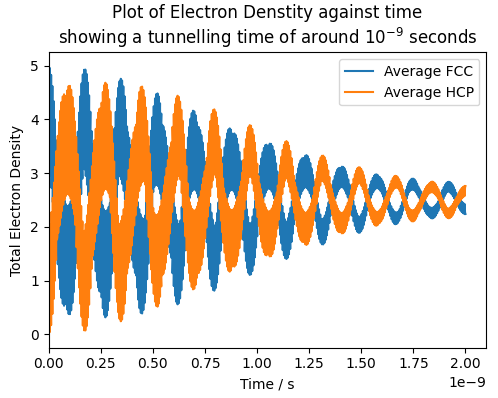
\includegraphics[width=0.9\linewidth]{Figures/Simulation/Plot of large band simulation decay times.png}
        \subcaption{Tunnelling excluding hydrogen energy}\label{fig:large band degenerate simulation}
    \end{subfigure}
    \hfill
    \begin{subfigure}{0.45\linewidth}
        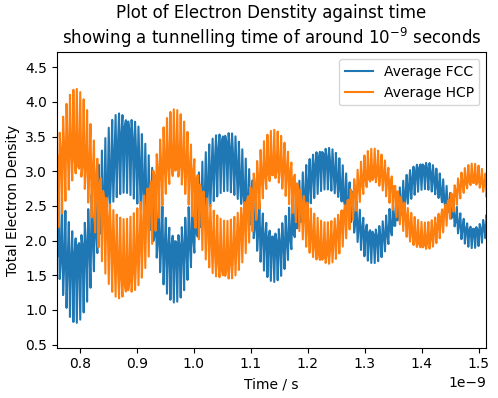
\includegraphics[width=0.9\linewidth]{Figures/Simulation/Plot of large band simulation decay times rapid oscillations.png }
        \subcaption{Rapid oscillation of the hydrogen occupation}
    \end{subfigure}
    \caption{Plot of the tunnelling rate taken using a
        simple choice of electron energies,
        taken evenly in the range \(E=E_f \pm 2 K_b T\).
        Simulation with a degenerate hydrogen
        (\cref{fig:large band degenerate simulation})
        shows tunnelling in around
        \(10^{-9}s\). TODO-Change title of plot}\label{fig:tunnelling rate single large band}
\end{figure}
Unfortunately we find that the interaction is
relatively large. The diagonal terms in
the interaction hamiltonian
had a value of \(6.21\times{}10^{-21}J\)
and a cross diagonal value of \(2.73\times{}10^{-23}J\)
whereas the electron energies were separated
by only \(9.2\times{}10^{-22}J\). This meant that
the perturbation approximation required for
fermi-dirac distributed states is not valid.
We also fail to see any tunnelling when
the hydrogen energy is included (\cref{fig:issues with single large band}).
\begin{figure}[htbp]
    \centering
    \begin{subfigure}{0.45\linewidth}
        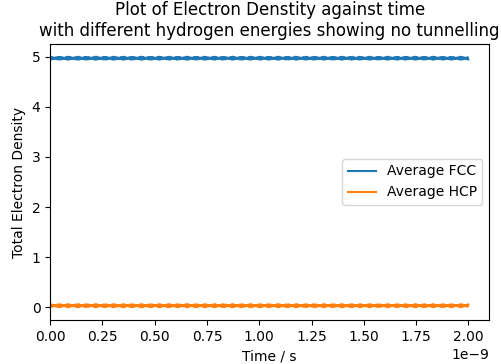
\includegraphics[width=0.9\linewidth]{Figures/Simulation/Plot of large band simulation with hydrogen energies.png}
        \subcaption{Tunnelling including hydrogen energy}\label{fig:large band non degenerate simulation}
    \end{subfigure}
    \hfill
    \begin{subfigure}{0.45\linewidth}
        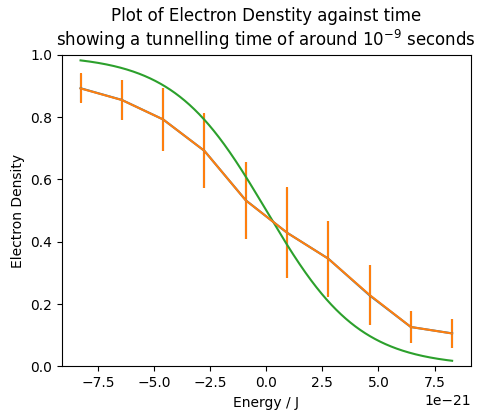
\includegraphics[width=0.9\linewidth]{Figures/Simulation/Plot of large band electron distribution.png}
        \subcaption{Electron Distribution}\label{fig:large band fermi-dirac}
    \end{subfigure}
    \caption{Plot demonstrating the issues with the
        simple approach used to calculate the rate.
        When including the hydrogen energies
        (\cref{fig:large band non degenerate simulation})
        no tunnelling can be seen, even
        at much larger timescales. Even without the
        inclusion of hydrogen energies
        the incorrect electron distribution is
        seen (\cref{fig:large band fermi-dirac}).
        TODO-Plot Title}\label{fig:issues with single large band}
\end{figure}

\subsection{Small Band Approach}\label{sec:small band approach}
To limit the effect of the incorrect
electron distribution we can
take electrons localised
in a small region of the fermi
surface such that their energies
and occupations are all similar.

One issue is that states at the edge
of the band will be `missing'
states to mix with during the
perturbation. We can approximate
this overlap using first order perturbation theory.
\begin{equation}
    \ket{n} = \ket{n^{(0)}} + \sum_{K\neq{}n} \frac{\bra{k^{(0)}} \hat{H}_{int} \ket{n^{(0)}}}{E_n^{(0)} - E_k^{(0)}} \ket{k^{(0)}}
\end{equation}
Since \(\hat{H}_{int} \propto E_{space}\)
(\cref{eqn:energy spacing dependance of interaction hamiltonian})
the degree of overlap of neighbouring states does
not depend on the energy spacing. Luckily
however the interaction is small
enough such that states only interact with
their closest neighbours (\cref{fig:single band energies}),
and the effect of these missing states should be small.
\begin{figure}[htbp]
    \centering
    \begin{subfigure}{0.45\linewidth}
        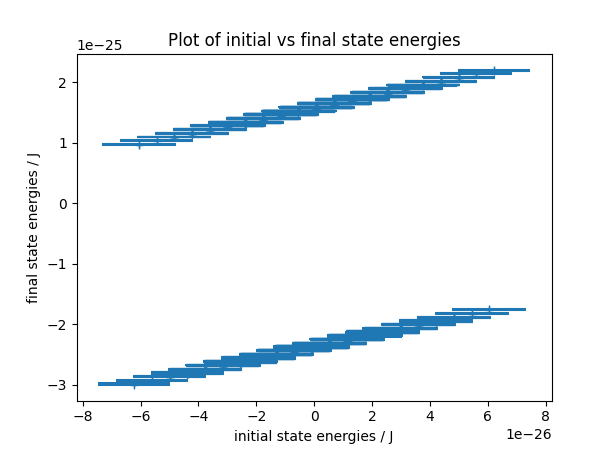
\includegraphics[width=0.9\linewidth]{Figures/Simulation/Plot of single band eigenstate energy range.png}
        \subcaption{Final State Energies}\label{fig:initial and final state energies of single band}
    \end{subfigure}
    \hfill
    \begin{subfigure}{0.45\linewidth}
        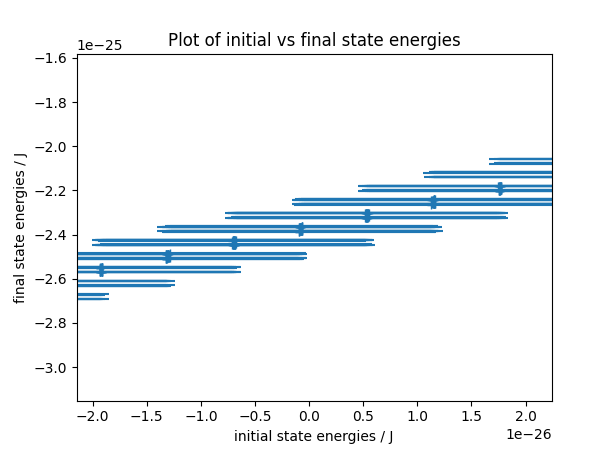
\includegraphics[width=0.9\linewidth]{Figures/Simulation/Plot of single band eigenstate energy range closeup.png}
        \subcaption{Detailed view of lower energies}\label{fig:initial and final state energies of single band zoom}
    \end{subfigure}
    \caption{Plot of average initial state energy weighted by the
        probability of occupation. The final
        state energy is separated into two,
        due to the symmetric and antisymmetric
        contributions
        (\cref{fig:initial and final state energies of single band}).
        In \cref{fig:initial and final state energies of single band zoom}
        we can see each state is highly degenerate, and mixing
        is limited to the four nearest neighbours.
    }\label{fig:single band energies}
\end{figure}


The tunneling could also be
influenced by these states
through a combination of
several electron `hops'.
Due to the energy time uncertainty
principle \(\Delta{}E\Delta{}T \geq \frac{\hbar}{2}\)
we expect the total energy to be conserved
to within
\begin{equation}
    \Delta{}E \sim \frac{\hbar}{2\Delta{} t}
\end{equation}
so that for a tunnelling time of
\(\sim 10^{-9}s\)
we expect an energy fluctuation
of \(\sim 5\times{}10^{-26} J\).
We therefore choose states separated
by at-least \(10^{-25} J\) such that
interaction with states outside
the band is prohibited
through energy conservation.


\subsection{Different Hydrogen Energy}\label{sec:different hydrogen energy}
If we add the hydrogen energies to the
simulation we no longer see tunnelling
on any timescale. Repeating the analysis
in \cref{sec:small band approach} we
see that eigenstate mixing and hence
tunnelling is dominated by
eigenstates degenerate in energy.
In the initial approach we therefore
miss many of the states which could
contribute to tunnelling. To ensure that we always have
states degenerate in energy we
therefore introduce two electron
bands separated by the hydrogen energy
difference.
\begin{figure}[htbp]
    \centering
    \begin{subfigure}{0.45\linewidth}
        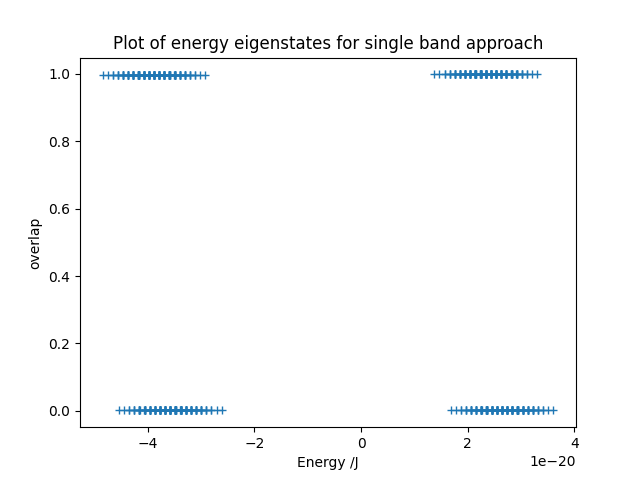
\includegraphics[width=0.9\linewidth]{Figures/Simulation/single band eigenstate energies.png}
        \subcaption{One Band Overlaps}\label{fig:one band overlap}
    \end{subfigure}
    \hfill
    \begin{subfigure}{0.45\linewidth}
        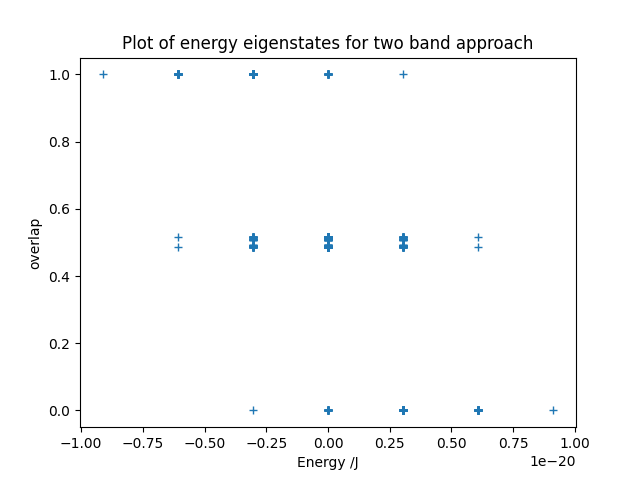
\includegraphics[width=0.9\linewidth]{Figures/Simulation/two band eigenstate energies.png}
        \subcaption{Two Band Overlaps}\label{fig:two band overlap}
    \end{subfigure}
    \caption{Plot of the energies of the
        eigenstates, against the portion of the
        state which lies in the FCC site.
        For the single band approach we
        see very little overlap between the FCC and HCP
        initial states (\cref{fig:one band overlap})
        as the energies of the FCC and HCP sites
        are poorly matched. By introducing
        two bands separated by the hydrogen energy
        difference (\cref{fig:two band overlap})
        we find mixing between states which are
        degenerate in energy
    }\label{fig:overlap with hydrogen energies}
\end{figure}

If we were to plot the initial and final
state energies for the single band approach
we no longer see two distinct levels. Instead
we see three levels split into
several distinct groups.
To promote interaction between each group
we could increase the width of each band,
however this leads to a reduction in
the overlap between states. This is
caused by different mixing
within each band which prevents
the energy degeneracy. To solve this
we could simply remove the diagonal
interaction, however in (\cref{sec:tunnelling no diagonal})
we find this effects the
measured tunneling times.
Even when
working with a small band
we do not see the desired equilibrium
behaviour, calculated assuming the rate
scales as \(N(1-N)\).
\begin{figure}[htbp]
    \centering
    \begin{subfigure}{0.45\linewidth}
        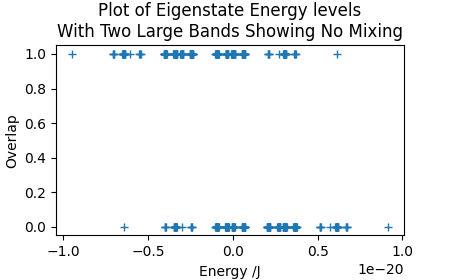
\includegraphics[width=0.9\linewidth]{Figures/Simulation/Two Large Bands No Mixing.png}
        \subcaption{Large Band Mixing}\label{fig:two band minimum mixing}
    \end{subfigure}
    \hfill
    \begin{subfigure}{0.45\linewidth}
        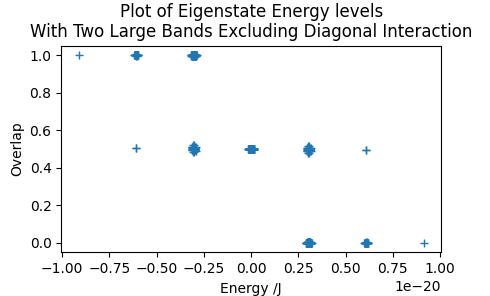
\includegraphics[width=0.9\linewidth]{Figures/Simulation/Two Large Bands No Diagonal.png}
        \subcaption{Large Band No Diagonal}\label{fig:two band no diagonal}
    \end{subfigure}
    \begin{subfigure}{0.45\linewidth}
        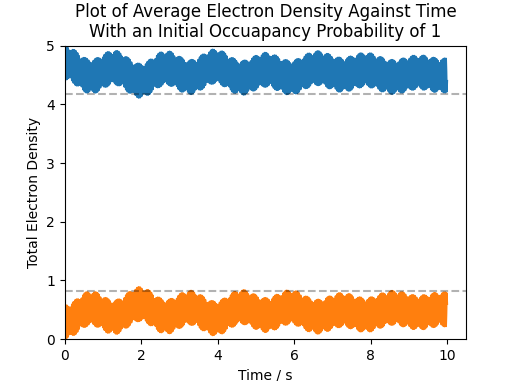
\includegraphics[width=0.9\linewidth]{Figures/Simulation/Two Small Bands Large Probability Incorrect Equilibrium.png}
        \subcaption{Large Initial Occupation}\label{fig:two band incorrect equilibrium above}
    \end{subfigure}
    \hfill
    \begin{subfigure}{0.45\linewidth}
        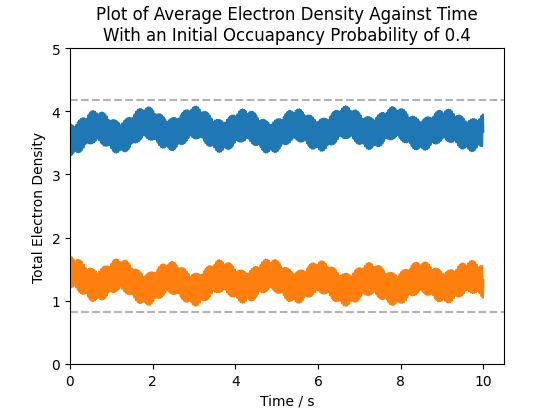
\includegraphics[width=0.9\linewidth]{Figures/Simulation/Two Small Bands Small Probability Incorrect Equilibrium.png}
        \subcaption{Small Initial Occupation}\label{fig:two band incorrect equilibrium below}
    \end{subfigure}
    \caption{
        Plots demonstrating the issues
        with the two band approach.
        \cref{fig:two band minimum mixing}
        demonstrates the issue with
        using a large band; the diagonal
        interaction causes mixing within
        groups of eigenstates which
        lifts the degeneracy required for
        the off diagonal interaction.
        This can be fixed by removing
        the diagonal interaction
        (\cref{fig:two band no diagonal})
        however in
        \cref{sec:tunnelling no diagonal}
        we find this is
        necessary for the correct
        tunneling behaviour.
        Even with a small band
        the
        predicted equilibrium
        behaviour is not seen
        (\cref{fig:two band incorrect equilibrium above,fig:two band incorrect equilibrium below}).
        There is therefore very
        little evidence that
        this method would
        approximate the true
        electron-hydrogen dynamics.
    }\label{fig:issue with two band approach}
\end{figure}
Interestingly we do see a reduction in
fluctuations if the system is initially
prepared with this occupation
(\cref{fig:two band close to equilibrium}).
We also find the material cools
as the hydrogen tunnels, as can be seen
through the average electron distribution in
the initial and final state. This is a
result of energy transfer from the
electron gas to the hydrogen
(\cref{fig:two band temperature shift}).

\begin{figure}[htbp]
    \centering
    \begin{subfigure}{0.45\linewidth}
        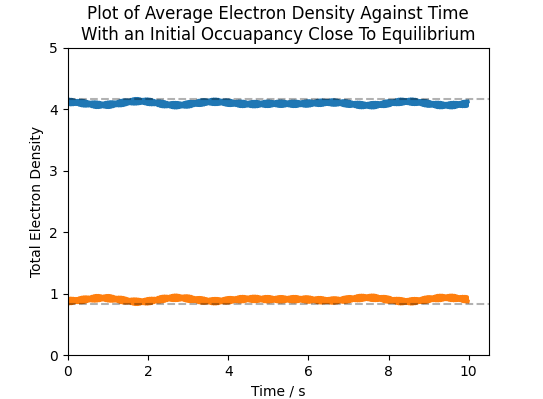
\includegraphics[width=0.9\linewidth]{Figures/Simulation/Two Small Bands Probability Clsoe To Equilibrium.png}
        \subcaption{Evoulution Close To Equilibrium}\label{fig:two band close to equilibrium}
    \end{subfigure}
    \hfill
    \begin{subfigure}{0.45\linewidth}
        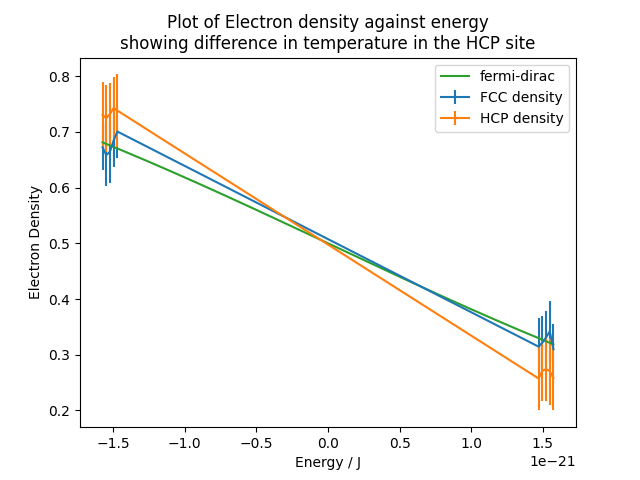
\includegraphics[width=0.9\linewidth]{Figures/Simulation/two band electron distribution.png}
        \subcaption{Two Band Electron Distribution}\label{fig:two band temperature shift}
    \end{subfigure}
    \caption{
        Interesting features of the two
        band dynamics.
        In \cref{fig:two band close to equilibrium}
        we find noise is reduced when the
        hydrogen is prepared in a state
        close to the predicted equilibrium
        occupation. This suggests it is
        true equilibrium of the
        system.
        In \cref{fig:two band temperature shift}
        the temperature shift can be seen.
        This is a consequence of energy transfer
        between the electron gas to the
        hydrogen. The temperature
        shift can be reduced by adding
        more electrons to the
        simulation.
    }\label{fig:final notes two band}
\end{figure}